\section{Contabilidad y finanzas}
\subsection{Autoevaluación}
En esta sección se ha cumplido los objetivos correspondientes al 10.
\subsection{Introducción}
\paragraph{}
Uno de los módulos esenciales para cualquier empresa es el módulo de finanzas y contabilidad. Este debe de ayudar a sus usuarios a gestionar sus beneficios y gastos, además de encargarse de automatizar labores administrativos como la declaración de la renta o la gestión de impuestos. En esta sección se busca analizar el problema del módulo FICO de Odoo y buscar una solución, que nos permite gestionar la contabilidad y finanzas desde nuestro ERP. Para ello hemos realizado un estudio detallado sobre la gestión contable y financiera en Odoo, centrándose en el contexto español. Se identifican los problemas del módulo FICO en Odoo, se propone una solución en la nube y se describe el proceso de integración con Odoo. Este estudio tiene como objetivo proporcionar una visión integral de las opciones disponibles para las PYMEs españolas en términos de contabilidad y finanzas.
\subsection{Metodología}
\paragraph{}
La metodología empleada se basa en una revisión exhaustiva de los problemas reportados en el repositorio de Github \href{https://github.com/OCA/l10n-spain/issues}{OCA/l10n-spain issues}, así como en la evaluación de diversas soluciones FICO en la nube. Odoo es un software Open Source, por lo que gran parte de las mejoras son realizadas por la comunidad, como en este caso. Este repositorio es de la comunidad española de Odoo, la cual busca cada día mejorar este ERP. También, se ha realizado un análisis comparativo de las posibles soluciones encontradas; considerando sus características, ventajas y aplicabilidad a las necesidades específicas del mercado español. Por último, se ha investigado como se puede llevar a cabo el proceso de integración entre Odoo y la solución FICO seleccionada, siguiendo pasos técnicos específicos.
\subsection{Resultados y análisis}
Tras analizar cual es el problema de este modulo nos hemos dado cuenta que existen varios problemas. El primer gran problema es que el soporte de este módulo en Odoo 17.0 es de pago además de estar incompleto. Otro gran problema es que si queremos utilizar Odoo en castellano muchas de sus funcionalidades no están migradas a este versión, por lo tanto, hay varios módulos que no se han implementado o están en proceso. Si queremos conocer cuales de los módulos son totalmente funcionales en la versión 17.0 podemos revisar el \textit{issue} del repositorio de Github \href{https://github.com/OCA/l10n-spain/issues/3298}{Migration to version 17.0}. Aquí encontraremos la información de los módulos que han sido migrados con éxito, cuales se está trabajando y cuales todavía no se pueden utilizar en castellano en la versión 17.0 de español. Analizando este lista podemos observar que a penas hay once ítems completados, de los 42 que se deben implementar. Otro problema que nos ha llamado la atención es el problema con las subvenciones. Un usuario de la comunidad ha creado un \textit{issue} reportando este problema. Sin embargo, el problema que más no ha llamado la atención es el problema con la \href{https://github.com/OCA/l10n-spain/issues/3527}{Gestión de IRPFs y sus posiciones fiscales}. En este \textit{issue} se describe el problema en la configuración de impuestos en Odoo. Actualmente no se garantiza que los impuestos se apliquen correctamente en función del tipo de entidad; autónomo o empresa, ni en el tipo de transacción, compra o venta.

\paragraph{}
Hemos decidido analizar los posibles software que nos ayuden a solucionar este problema. Y una vez que hayamos encontrado esta solución la conectaremos a nuestro ERP mediante conectores que nos proporciona Odoo. Existen API públicas que nos permiten conectar módulos externos al nuestro. En este caso vamos a buscar un módulo específico de finanzas que tengan herramientas que nos aporten un valor diferencial al resto. 

\paragraph{}
Los dos gestores de finanzas que hemos decidido analizar son: 

\begin{itemize}
    \item \href{https://www.sage.com/es-es/software-contabilidad/}{Sage Business Cloud Contabilidad}: Sage ofrece una gama de soluciones de contabilidad y gestión empresarial que pueden adaptarse a las necesidades específicas de autónomos y empresas. Su software de contabilidad en la nube permite gestionar impuestos, facturación, compras y ventas de manera integrada y personalizable.

    \item \href{https://quickbooks.intuit.com/es/}{QuickBooks}: QuickBooks es un software de contabilidad popular que ofrece soluciones para autónomos y pequeñas empresas. Permite configurar impuestos y posiciones fiscales de manera flexible, adaptándose a las necesidades específicas de cada usuario. Además, ofrece herramientas para gestionar facturas, gastos, y otros aspectos financieros de manera eficiente.
\end{itemize}

\paragraph{}
Tras realizar un análisis exhaustivo hemos llegado a las siguientes conclusiones: 
\begin{enumerate}

\item \textbf{Funcionalidad y Flexibilidad}:
   \begin{itemize}
       \item Sage Business Cloud Contabilidad ofrece una amplia gama de funciones para la gestión contable, incluyendo herramientas para gestionar impuestos, facturación, compras y ventas. Su plataforma en la nube permite una personalización significativa para adaptarse a las necesidades específicas de los usuarios.
       \item QuickBooks también proporciona una variedad de funciones contables esenciales, como la gestión de impuestos, facturación y seguimiento de gastos. Su interfaz intuitiva y opciones de personalización hacen que sea fácil de usar para autónomos y pequeñas empresas.
   \end{itemize}

\item \textbf{Facilidad de Uso}:
   \begin{itemize}
       \item Sage Business Cloud Contabilidad puede resultar un poco más complejo para usuarios nuevos debido a su amplia gama de funciones y opciones de personalización. Sin embargo, una vez familiarizado con la plataforma, ofrece un flujo de trabajo fluido y eficiente.
       \item QuickBooks se destaca por su interfaz intuitiva y fácil de usar, lo que lo convierte en una excelente opción para usuarios que buscan una solución contable simple y directa.
   \end{itemize}

\item \textbf{Soporte al Cliente}:
   \begin{itemize}
       \item Sage Business Cloud Contabilidad ofrece soporte técnico a través de varios canales, incluyendo chat en vivo, correo electrónico y recursos en línea como tutoriales y documentos de ayuda.
       \item QuickBooks también proporciona un sólido soporte al cliente a través de chat en vivo, correo electrónico y una extensa base de conocimientos en línea.
   \end{itemize}

\item \textbf{Precio}:
   \begin{itemize}
       \item Los precios de Sage Business Cloud Contabilidad varían según el plan y las necesidades específicas del usuario, con opciones de suscripción mensual o anual.
       \item QuickBooks ofrece diferentes planes de precios para adaptarse a diferentes tamaños de empresa y necesidades de contabilidad, con opciones de suscripción mensual.
   \end{itemize}

\end{enumerate}

\paragraph{}
Ambas opciones tienen sus ventajas y sus desventajas, considerando nuestras necesidades y lo que nos ofrece cada uno hemos decidido elegir Sage Business Cloud. A pesar de su mayor precio consideramos que la plataforma en la nube es vital para nosotros. Además, al ser un ERP más grande siempre va a tener una mayor cantidad de recursos y comunidad detrás. Para su integración con nuestro ERP vamos a utilizar un módulo denominado \href{https://apps.odoo.com/apps/modules/14.0/odoo_sage_integration/}{Sage Integration}. Este módulo nos permite sincronizar Sage con Odoo de una forma muy sencilla. Debemos instalar este módulo en nuestro ERP y crearnos una cuenta en \textit{Sage Developer Accounting}. Después, debemos crear una nueva aplicación y rellenar el formulario. Se nos proporcionará unas credenciales, las cuales deberemos utilizar en el módulo instalado. Seguiremos las pasos que nos indica y tendremos conectado ambos ERP.
En la Figura \ref{fico} podemos ver el proceso de integración de forma visual.

\begin{figure}
    \centering
    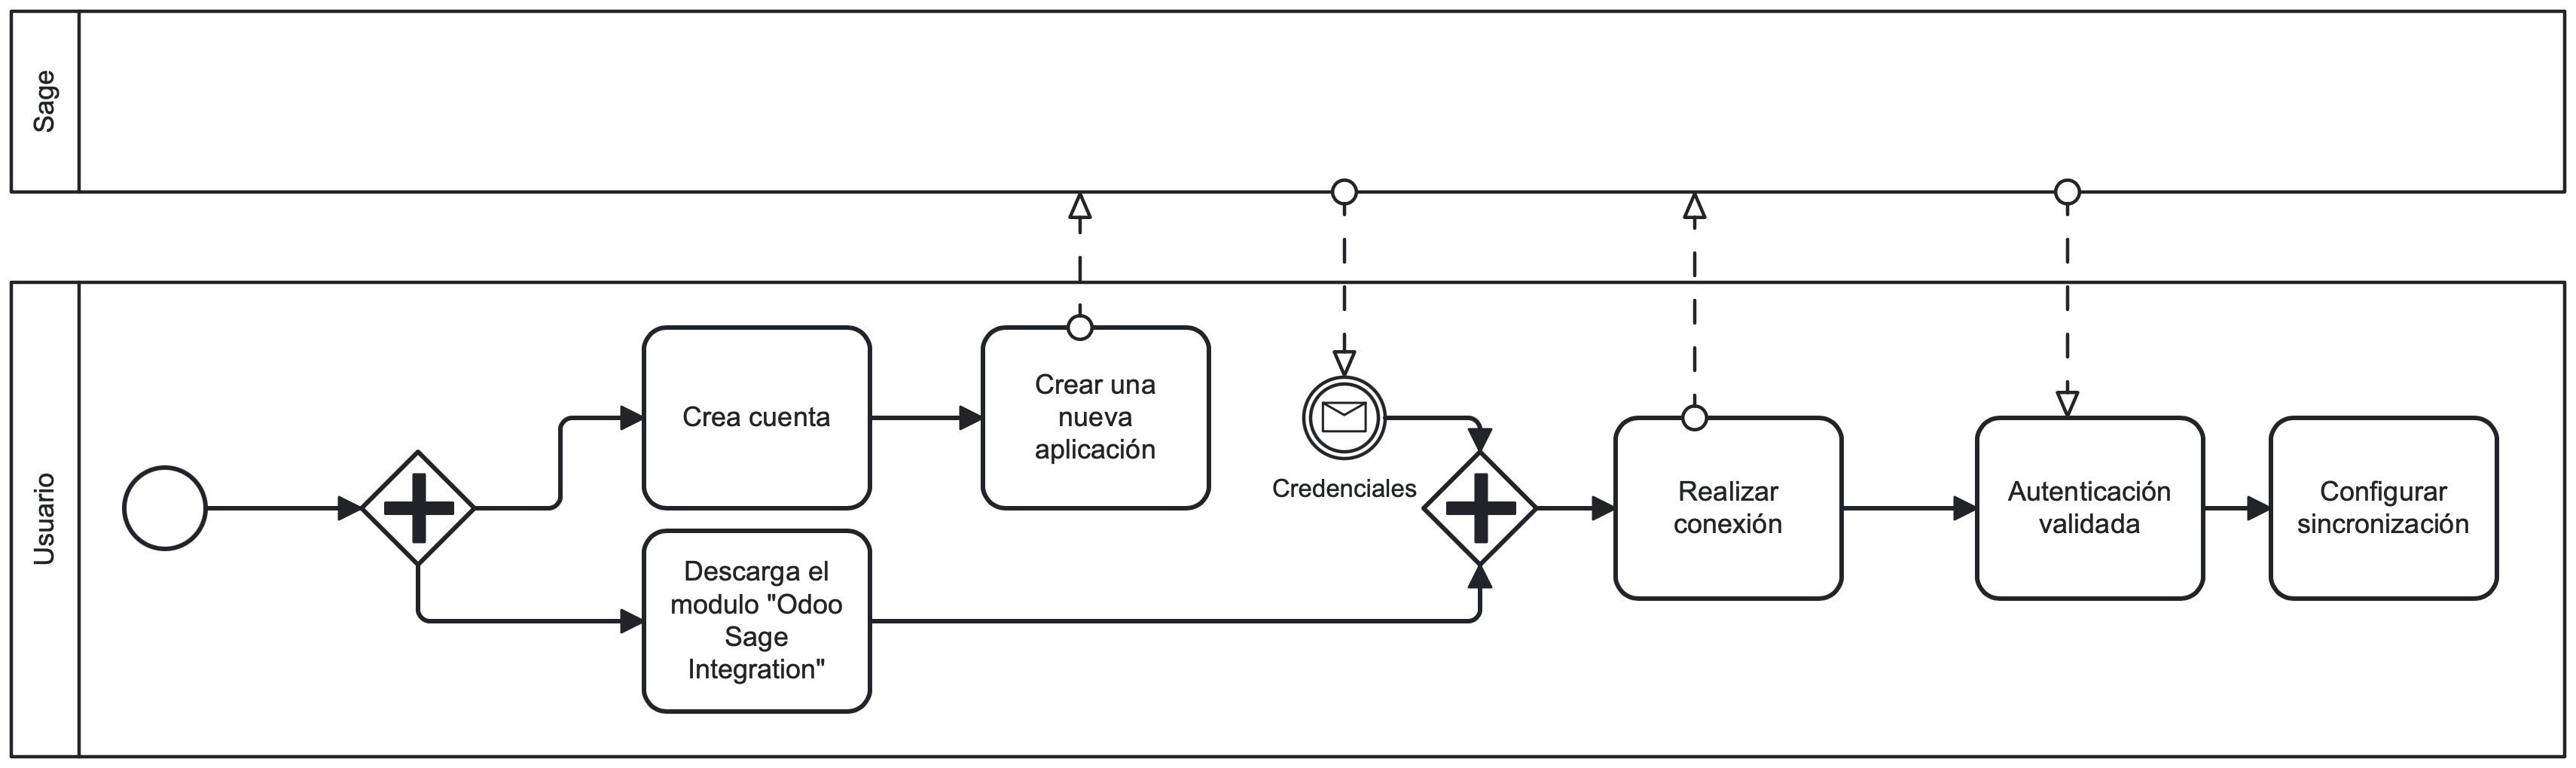
\includegraphics[width=1\linewidth]{imgConta/Fico.png}
    \caption{Diagrama BPMN 2.0 del proceso de integración de Odoo Y Sage Business Cloud}
    \label{fico}
\end{figure}

\subsection{Conclusiones}
Tras analizar el problema y las posibles soluciones externas podemos concluir:
\subsection{Conclusiones}
\paragraph{}
Basándonos en el análisis detallado realizado, las conclusiones se derivan de los siguientes puntos clave:

\begin{enumerate}
    \item \textbf{Problemas Identificados en el Módulo FICO de Odoo:} Tras un análisis exhaustivo, se han identificado varios problemas en el módulo FICO de Odoo, destacando la limitada disponibilidad de soporte para la versión 17.0, la incompletitud de la migración a español, y problemas específicos como la gestión de subvenciones y la configuración de impuestos, particularmente el IRPF. Estos problemas impactan la funcionalidad y la confiabilidad del módulo para usuarios en el contexto español.
    
    \item \textbf{Selección de Soluciones Alternativas:} Con el objetivo de resolver los problemas identificados, se han evaluado dos soluciones externas: Sage Business Cloud Contabilidad y QuickBooks. Ambas opciones ofrecen funcionalidades esenciales para la gestión contable y financiera, así como opciones de personalización. Sin embargo, se destaca la mayor complejidad de Sage Business Cloud Contabilidad y la intuitividad de QuickBooks.
    
    \item \textbf{Elección de Sage Business Cloud Contabilidad:} Después de considerar los factores mencionados, se ha decidido seleccionar Sage Business Cloud Contabilidad como la solución preferida. A pesar de su precio relativamente más alto, se valora su plataforma en la nube y el respaldo de una comunidad más amplia, lo que proporciona recursos adicionales y una mayor seguridad en la integración con el ERP existente.
    
    \item \textbf{Proceso de Integración:} Para facilitar la integración con Odoo, se utilizará el módulo Sage Integration, que simplifica la sincronización entre ambas plataformas. Se seguirán los pasos detallados proporcionados por la herramienta para establecer una conexión fluida y efectiva entre Sage Business Cloud Contabilidad y el ERP Odoo.
\end{enumerate}
\paragraph{}
En resumen, la selección de Sage Business Cloud Contabilidad como solución alternativa para los problemas identificados en el módulo FICO de Odoo se basó en una evaluación cuidadosa de las características, funcionalidades y compatibilidad con los requisitos específicos del contexto español. La elección se respalda en la confianza en la plataforma en la nube y en la comunidad detrás de Sage, así como en la facilidad de integración proporcionada por el módulo Sage Integration.
